\chapter{Monte-Carlo}

Monte-Carlo Experimente bezeichnen eine Klasse von Algorithmen, 
welche durch wiederholtes generieren von Zufallszahlen ein Problem numerisch approximieren.
Diese Algorithmen können unter anderem genutzt werden, um besonders schwierige Probleme zu lösen,
welche auf analytischem Wege unmöglich wären.

Ein Beispiel einer Monte-Carlo Methode wurde in dieser Vorlesung bereits für die \link{algo:av-methode}{Annahme-Verwerfungs-Methode} eingesetzt.
In diesem Fall konnte durch das zufällige Generieren von Punkten die potenziell schwierige \link{algo:inv-methode}{Inversionsmethode} umgangen werden.
\\
\begin{wrapfigure}{r}{0.5\textwidth}
\centering
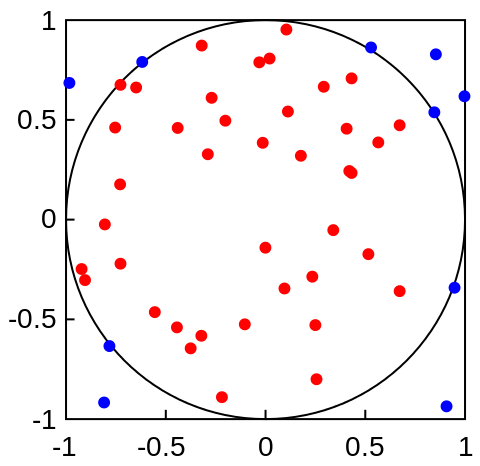
\includegraphics[width=0.4\textwidth]{mc-integration}
\end{wrapfigure}

Solche Simulationen sind anhand eines Beispiels leicht vorstellbar.
Es gibt eine quadratische Fläche, in welcher sich ein runder Pool befindet.
Wenn nun an zufälligen Stellen Golfbälle fallen gelassen werden, so landen diese entweder innerhalb oder außerhalb des Pools.
Wird nun die Menge der im Pool gelandeten Bälle mit der außerhalb gelandeten ins Verhältnis gesetzt,
so kann der Flächeninhalt des Pools ermittelt werden.
Dieser Algorithmus kann für Objekte beliebiger Komplexität und Dimensionalität angewendet werden.

\section{Numerische Integration}

Gegeben sei eine beliebige stückweise stetige Funktion:

\[f(x) \in (0, \infty) \qquad x \in [a,b]\]

Gesucht ist der Flächeninhalt von $f(x)$ im Intervall $[a,b]$.
Hierfür wird zuerst ein Rechteck mit Breite $b-a$ und Höhe $K = \max(f(x))$ bestimmt.
Nun kann das Verhältnis zwischen Rechteck und der Fläche unter dem Funktionsgraphen folgendermaßen als Wahrscheinlichkeit beschrieben werden:

\[p = \frac{I}{K(b-a)}\]

wobei $I$ das Integral der Funktion ist.
Wird diese Gleichung nach $I$ umgestellt und die Variablen $I,p$ mit ihren approximierten Variablen $\hat{I},\hat{p}$ ersetzt,
so entsteht die allgemeine Formel für den approximierten Flächeninhalt:

\[\hat{I} = K(b-a)\hat{p}\]

\subsection{Algorithmus A}

Diese Gleichung kann sehr einfach, 
aufbauend auf der \link{algo:av-methode}{Annahme-Verwerfungs-Methode},
angewendet werden.
Zuerst werden $N$ Iterationen der AVM durchgeführt und die Menge generierter Zahlen $A$ ermittelt.
Nun können $\hat{p}$, sowie $\hat{I}$ als: 

\[\hat{p} = \frac{A}{N}\]
\[\hat{I} = K(b-a)\hat{p}\]

bestimmt werden.

\subsection{Algorithmus B}

Der nächste Algorithmus wird folgendermaßen hergeleitet:

\[I = \int_a^b f(x)dx = 
\int_{-\infty}^\infty f(x)(b-a)
\frac{1}{(b-a)}\mathds{1}_{[a,b]}(x)\]

\[g(x) := f(x)(b-a)\]

\[\hat{I} = \frac{g(U_1) + ... + g(U_n)}{n}\]

Hierdurch entsteht die folgende nützliche Gleichung:

\[\hat{I} = (b-a)\frac{(f(U_1) + ... + f(U_n))}{n}\]

Diese kann intuitiv als \textbf{durchschnittlicher Wert von f(x)} multipliziert mit \textbf{Breite des Intervalls} bezeichnet werden.
Die Funktion wird also mithilfe des arithmetischen Mittels durch eine Gleichverteilung angenähert und dessen Integral als Rechteck berechnet.



\begin{algorithm}[h!]
    \DontPrintSemicolon
    \LinesNumbered
    
    Setze $A=0$\;
    \For(){k=1; k<N}{
      Erzeuge $x\sim U(a,b)$\;
      Setze $A=A+f(x)$\;
    }
    Setze $\hat{I} = \frac{(b-a)}{N}A$
    
    
    \caption{Algorithmus B}\label{algo:algo-b}
\end{algorithm}


% #############################################

% Ich bin mir ziemlich sicher Algo C hab ich hier falsch beschrieben.
% Ist zum Glück nicht Prüfungsrelevant

% #############################################

% \subsection{Algorithmus C}

% Der letzte Algorithmus orientiert sich an der Methode des \link{algo:imp-samp}{Importance Sampling}.
% Hier wird wieder eine Hilfsfunktion genutzt, welche es ermöglicht leicht (Inversionsmethode) Zufallszahlen zu generieren.
% Diese Zahlen werden dann anstelle der Uniformverteilung aus Algorithmus B genutzt um gezielter Punkte zu ermitteln.
% Um die dadurch veränderte Verteilung der Punkte muss zum Schluss nur noch ausgeglichen werden, 
% indem der Parameter $A$ um das Verhältnis der Funktion $f(x)$ und der Hilfsfunktion $\delta(x)$ inkrementiert wird. 
% Dieses Vorgehen ist im folgenden Algorithmus leicht zu erkennen:

% \begin{algorithm}[h!]
%   \DontPrintSemicolon
%   \LinesNumbered
  
%   Setze $A=0$\;
%   \For(){k=1; k<N}{
%     Erzeuge $x\sim \delta_x$\;
%     Setze $A=A+\frac{f(x)}{\delta_x(x)}$\;
%   }
%   Setze $\hat{I} = \frac{(b-a)}{N}A$
  
  
%   \caption{Algorithmus C}\label{algo:algo-c}
% \end{algorithm}

\section{Das Gesetz der großen Zahlen}

Das GGZ besagt, dass ein durch wiederholte Zufallsexperimente generierter Wert ebenfalls eine Zufallsvariable ist.
Ein Beispiel hierfür ist die Berechnung des arithmetischen Mittels aus $n$ einzelnen generierten Werten.

\[\overline{X}_n = \frac{1}{n}\sum^n_{i=1}X_i\]

Diese neue Zufallsvariable hat einen eigenen Erwartungswert und eine Varianz:

\[E(\overline{X}_n) = \mu_x\]
\[Var(\overline{X}_n) = \frac{\sigma}{n}\]

Der Erwartungswert entspricht also dem der ursprünglichen Verteilung und die Varianz sinkt mit steigender Zahl von Zufallsexperimenten.

\section{Der zentrale Grenzwertsatz}

Der zentrale Grenzwertsatz besagt, dass der Erwartungswert einer Zufallszahl für große $n$ Normalverteilt:

\[\overline{X}_n \approx N(\mu, \frac{\sigma^2}{n})\]

Abweichungen des Erwartungswertes können also mit den gleichen Methoden bestimmt und geschätzt werden, wie bei der Normalverteilung.
Bei solchen Problemstellungen existieren drei Variablen, welche die Genauigkeit beschreiben:

\begin{align*}
  \alpha&\: ...\: \text{Risikoschwelle}\\
  n&\: ...\: \text{Zahl der Wiederholungen}\\
  \epsilon&\: ...\: \text{Genauigkeit}\\
\end{align*}

Wenn in Aufgabenstellungen zwei dieser gegeben sind, ist es möglich die fehlende Variable zu bestimmen:

\begin{align*}
  \text{Geg.:}
  &n, \epsilon\\
  \alpha &\ge 2-2\phi\left(\frac{\epsilon\sqrt{n}}{\sigma}\right)\\
  \text{Geg.:}
  &\alpha, \epsilon\\
  n &\ge \left(Z_{1-\frac{\alpha}{2}}\frac{\sigma}{\epsilon}\right)^2\\
  \text{Geg.:}
  &n, \alpha\\
  \epsilon &\ge Z_{1-\frac{\alpha}{2}}\frac{\sigma}{\sqrt{n}}\\
\end{align*}

Hierbei ist $Z_{1-\frac{\alpha}{2}}$ das Quantil mit dem Wert $1-\frac{\alpha}{2}$.

\section{Der Satz von Moivre-Laplace}

Ist $Y$ Binominalverteilt $Y \sim B(n,p)$ und sind $np$ und $n(1-p)$ groß, so kann die Binomialverteilung durch eine Normalverteilung angenähert werden.
Die Parameter sind dann:

\[\mu = np \qquad \sigma^2=np(1-p)\]

Außerdem muss bei der Rechnung mit dieser Normalverteilung noch eine Stetigkeitskorrektur von $0.5$ eingefügt werden:

\[P(a < Y \le b) \approx 
  \phi\left(\frac{b+\mathbf{0.5}-np}{\sqrt{np(1-p)}}\right) - 
  \phi\left(\frac{a+\mathbf{0.5}-np}{\sqrt{np(1-p)}}\right)\]

Die Faustregel für die Gültigkeit dieser Regel lautet:

\[np(1-p) \ge 9\]

% VL 08 beinhaltet den gleichen Stoff wie 7 + Anwendung und Beispiele